\documentclass{beamer}
\usetheme{Copenhagen}
\usecolortheme{beaver} 

\title{Python in a physics lab}
\author{Gergely Imreh}
\date{PyCon Taiwan \\ \today}


\begin{document}

\maketitle

\section{Lab overview}

\begin{frame}{Lab overview}

\begin{figure}[ht]
	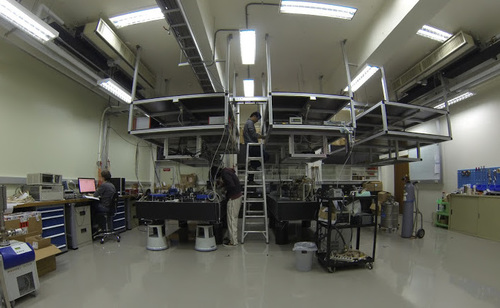
\includegraphics[width=10cm]{Labcrop500o.jpg}
\end{figure}


\end{frame}

\section{Experiment X}

\begin{frame}{Experiment X}

 \textbf{Laundry list of an experiment}
 
 \begin{itemize}
  \item Planning and theory
  \item Instrument control
  \item Interface
  \item Analysis and archiving
 \end{itemize}

\end{frame}

\subsection{Preparation}

\begin{frame}{Theory}

\textbf{Tools of theory:}

\begin{itemize}
	\item Numpy - Numerical Python
	\item SciPy - Scientific Python
	\item SymPy - Symbolic Math
	\item QuTIP$^2$ - Quantum Toolkit
	\item multiprocessing
	\item FreeCAD
\end{itemize}

\begin{figure}[ht]
	
\includegraphics[width=7cm]{numerical.png}
\end{figure}

\end{frame}


\subsection{Talking to instruments}

%\begin{frame}{Talking to instruments}
%
%
%
%\end{frame}

\begin{frame}[fragile]

\textbf{Serial}

\begin{verbatim}
import serial
instrument = serial.Serial("/dev/ttyUSB0",
                           baudrate=19200,
                           timeout=1)
instrument.write(cmd)
\end{verbatim}

\begin{figure}[ht]
	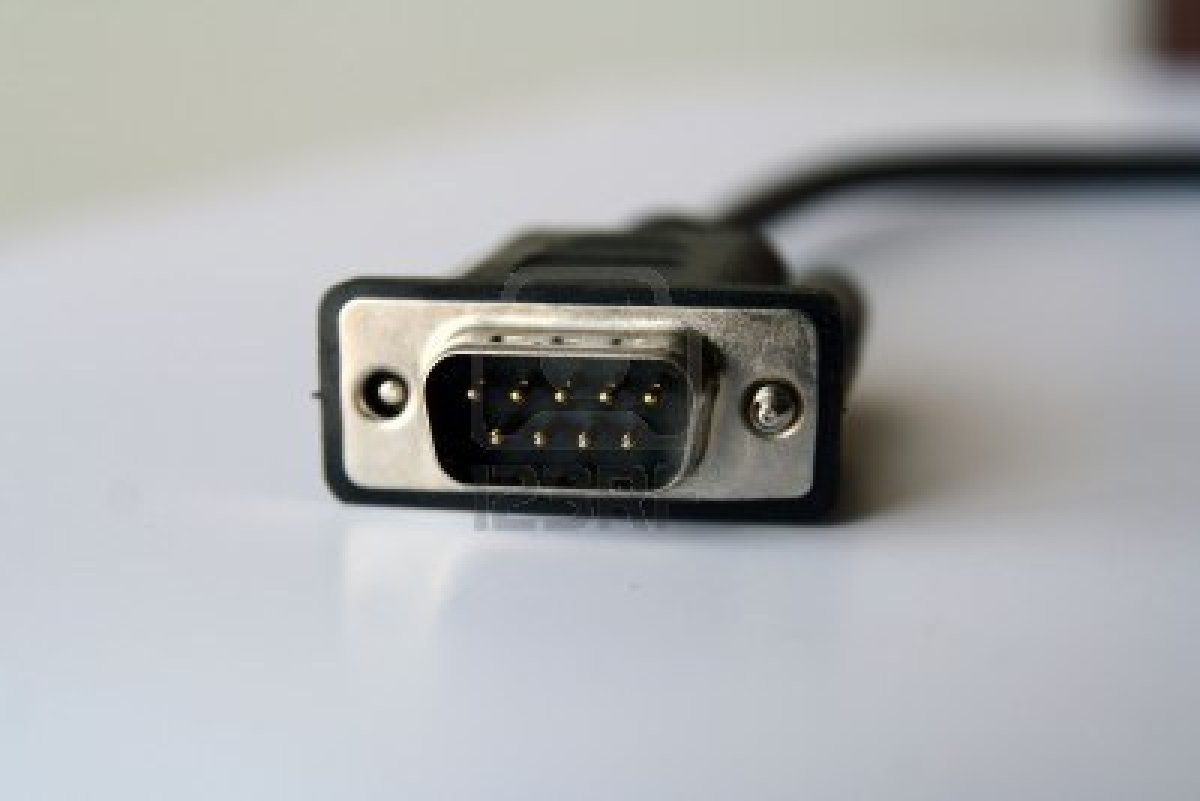
\includegraphics[width=8cm]{serial-connector.jpg}
\end{figure}
     
\end{frame}

\begin{frame}

\begin{figure}[ht]
	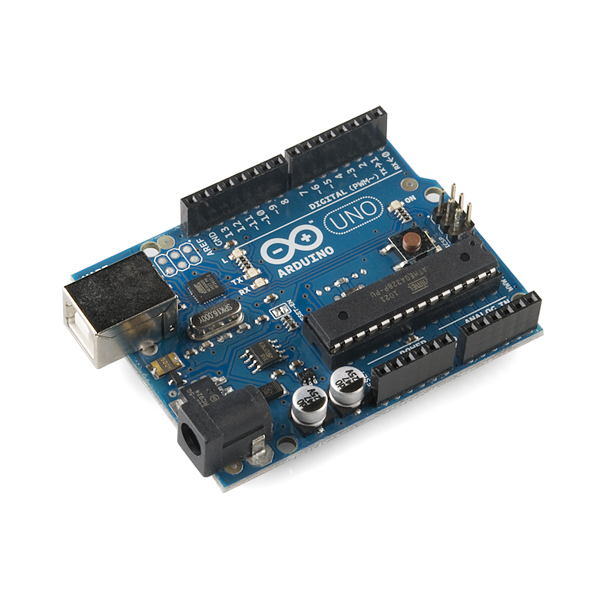
\includegraphics[width=8cm]{arduino.jpg}
\end{figure}

\end{frame}

\begin{frame}[fragile]

\textbf{GPIB: General Purpose Interface Bus}

\begin{verbatim}
import visa
oscilloscope = visa.instrument("GPIB::12")
print oscilloscope.ask("*IDN?")
\end{verbatim}

\begin{figure}[ht]
	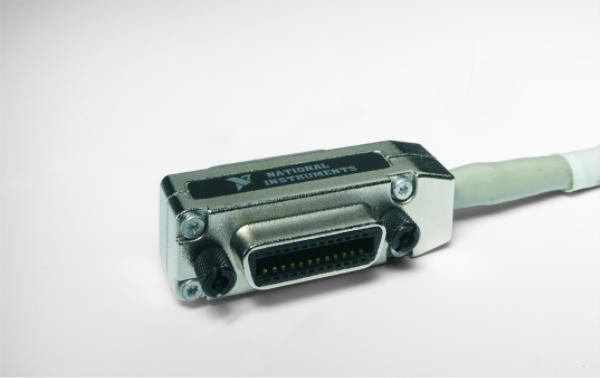
\includegraphics[width=8cm]{gpib1.JPG}
\end{figure}

\end{frame}

\begin{frame}

\begin{figure}[ht]
	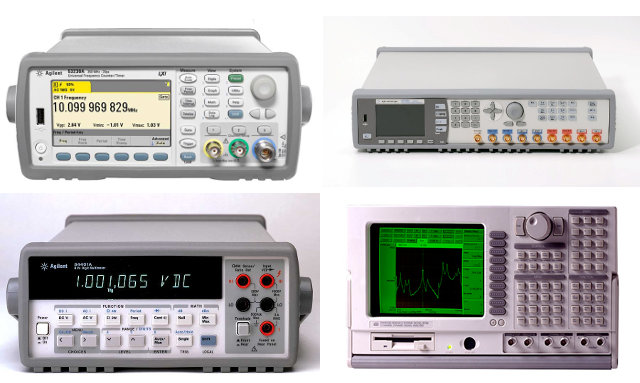
\includegraphics[width=10cm]{instruments.png}
\end{figure}

\end{frame}

\begin{frame}[fragile]

\textbf{FireWire IEEE-1394}

\begin{verbatim}
import pydc1394
lib = pydc1394.DC1394Library()
cams = l.enumerate_cameras()
cam0 = fw.Camera(l, cams[0]['guid'], isospeed=800)
image = numpy.array(cam0.current_image, dtype='f')
\end{verbatim}

\begin{figure}[ht]
	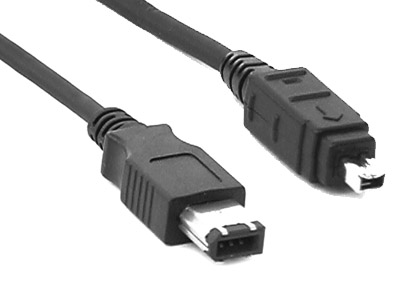
\includegraphics[width=6cm]{firewire.jpg}
\end{figure}

\end{frame}

\begin{frame}[fragile]

\textbf{ctypes}

\begin{verbatim}
import ctypes
my_dll = ctypes.windll.dll_name
receive_data = my_dll.ReceiveData
receive_data.restype = ctypes.c_long
\end{verbatim}

\begin{figure}[ht]
	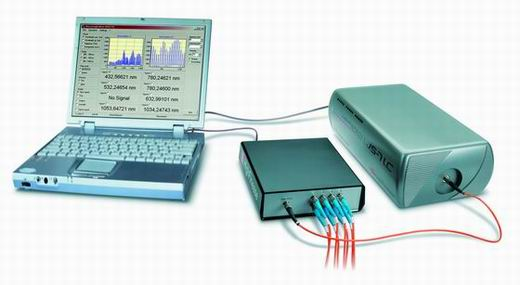
\includegraphics[width=8cm]{wlm.jpg}
\end{figure}

\end{frame}

%%%%%%%%
\begin{frame}[fragile]

\textbf{USB Test and Measurement Class}
\begin{verbatim}
import os
file = os.open(device, os.O_RDWR)
os.write(file, command)
\end{verbatim}

\begin{figure}[ht]
	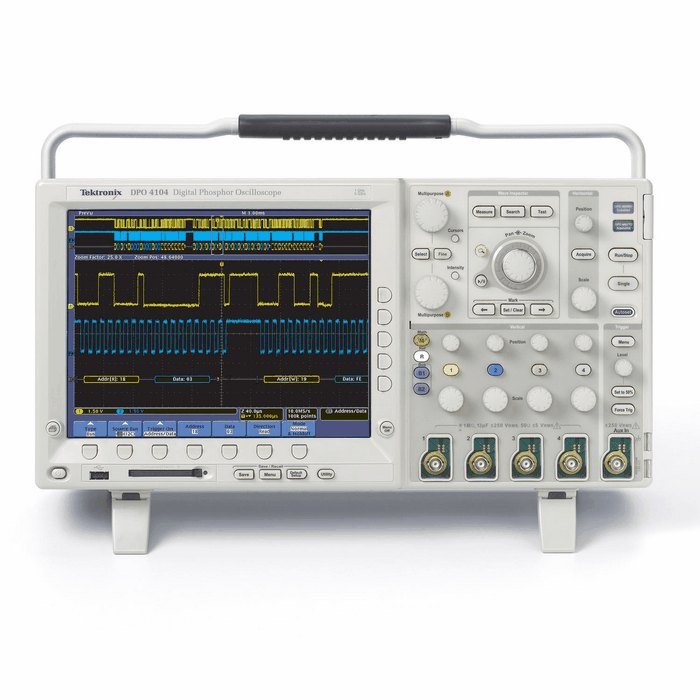
\includegraphics[width=6cm]{tek.jpg}
\end{figure}

\end{frame}

%%%%%%%%
\begin{frame}[fragile]

\textbf{PyMCU}

\begin{verbatim}
import pymcu
board = pymcu.mcuModule()
board.pinHigh(1)
board.pausems(500)
board.pinLow(1)
board.pausems(500)
\end{verbatim}

\begin{figure}[ht]
	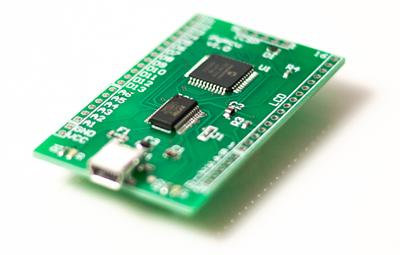
\includegraphics[width=6cm]{pymcu.jpg}
\end{figure}

\end{frame}


\subsection{Interface}

\begin{frame}{Interface}

\textbf{Tools of control}

\begin{itemize}
 \item WxPython
 \item PyGTK
 \item Bottle
 \item good ol' scripting
 \item PyGame
\end{itemize}


\end{frame}

\subsection{Analysis}

\begin{frame}[fragile]{Analysis}

\textbf{Tools of analysis:}

%\begin{itemize}
% \item NumPy - analysis
% \item Scipy - fitting
% \item Matplotlib - plotting
% \item PyTables - data
%\end{itemize}

\begin{figure}[ht]
	
\includegraphics[width=8cm]{analysis.png}
\end{figure}

\end{frame}

\begin{frame}[fragile]

\textbf{Matplotlib aka. pylab}

\begin{verbatim}
import pylab
import numpy
data = numpy.loadtxt(filename)
pylab.figure()
pylab.plot(data[:, 0], data[:, 0])
pylab.show()
\end{verbatim}

\begin{figure}[ht]
	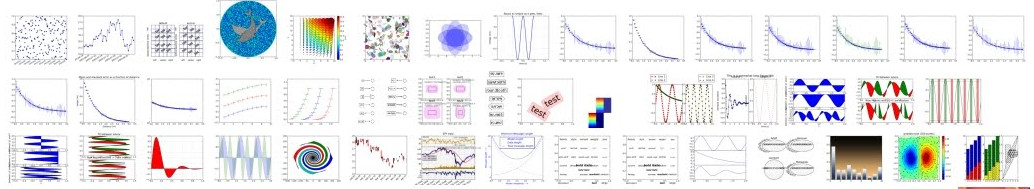
\includegraphics[width=11cm]{matplotlib_examples.jpg}
\end{figure}

\end{frame}

\section{Verdict}

\begin{frame}{Competitors}

\begin{figure}[ht]
	
\includegraphics[width=8cm]{competitors.png}
\end{figure}

\end{frame}

%\begin{frame}{Balance}
%\begin{figure}[ht]
%	
\includegraphics[width=10cm]{python-logo.png}
%\end{figure}
%\end{frame}


\begin{frame}[fragile]

\textbf{imrehg@gmail.com}

https://gergely.imreh.net

https://github.com/imrehg

\begin{figure}[ht]
	
\includegraphics[width=3cm]{Oxford_Logo.png}
	
\includegraphics[width=3cm]{Sinica_Logo.png}
	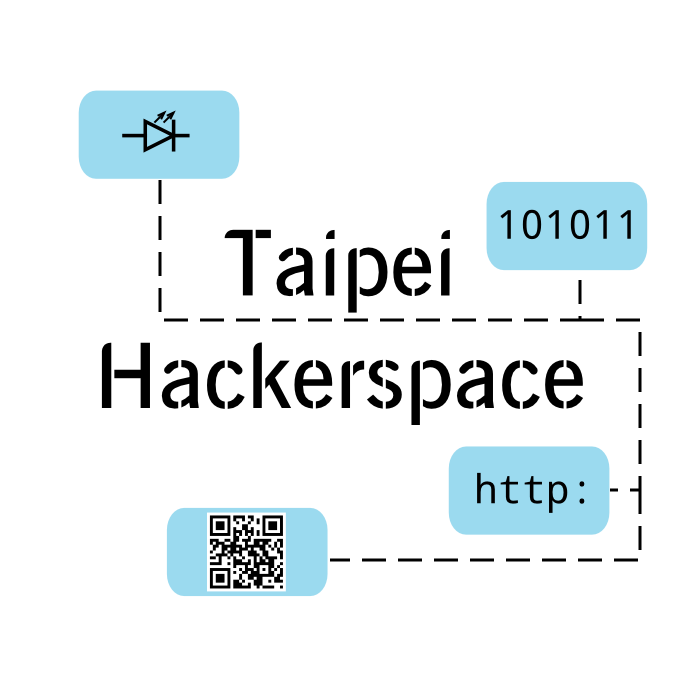
\includegraphics[width=3.5cm]{Hackerspace_Logo.png}
\end{figure}


\end{frame}


\end{document}